\chapter[Overview]{Overview of the Project}


\section{Introduction}

The rapid evolution of software development has increased demand for efficient design tools. UML diagrams serve as essential visual representations bridging conceptual design and implementation, facilitating stakeholder communication and providing standardized documentation approaches \cite{uml_importance}.

Traditional diagramming approaches present productivity barriers through manual effort and technical complexity. AI and natural language processing technologies have opened possibilities for automating diagram generation, transforming how developers create visual system representations \cite{ai_diagramming}.

This project addresses the need for an intelligent platform combining textual diagram precision with natural language accessibility, democratizing UML creation while maintaining professional standards.

\section{Overview of the Host Organization}
% This section will be completed later as requested

\section{Presentation of the Project Context}

\subsection{Problem Statement}

UML diagram creation faces challenges across GUI-based tools and textual specification languages.

\textbf{GUI-Based Tool Challenges:}

Traditional graphical tools present steep learning curves, time-consuming manual positioning, collaboration difficulties, and poor version control integration \cite{gui_limitations}. These limitations impact productivity and create inconsistencies across projects.

\textbf{Textual Tool Challenges:}

Tools like PlantUML and Mermaid require specific syntax knowledge, creating barriers for non-technical users \cite{plantuml_guide}. Complex error debugging and lack of real-time feedback slow the design process.

\textbf{Workflow Integration Issues:}

Both approaches suffer from poor development workflow integration, limited automation capabilities, and inadequate collaboration features \cite{workflow_integration}.

\subsection{Existing Solutions}

Several platforms address textual diagram generation challenges through different approaches.

\textbf{AI-Powered Platforms:}

Diagramming AI tools utilize artificial intelligence to interpret natural language and generate diagrams \cite{diagramming_ai}. These provide conversational interfaces and multi-format support but often lack precision for professional development.

\textbf{Conversational Tools:}

ChatUML and similar tools focus on natural language processing through chat interfaces \cite{chatuml}. They excel at simple diagrams and provide immediate feedback but struggle with complex enterprise requirements.

\textbf{Current Limitations:}

Existing solutions lack comprehensive AI integration, limited community features, and inconsistent output quality that falls short of professional standards \cite{existing_tools_analysis}.

\subsection{Proposed Solution}

Our platform addresses identified challenges through intelligent diagram generation that integrates AI with textual specification technologies.

\textbf{Core Innovation:}

The platform uses natural language processing to interpret user requirements and automatically generate UML diagrams \cite{nlp_diagramming}. By combining PlantUML precision with conversational interfaces, we eliminate traditional barriers.

\textbf{Key Features:}

Intelligent requirement interpretation processes natural language descriptions to identify entities and relationships, generating appropriate PlantUML code. Dynamic generation allows conversational refinement with real-time validation ensuring UML standard compliance \cite{plantuml_standards}.

Collaboration features enable team-based development with version control, while a community marketplace facilitates template sharing and knowledge exchange.

\textbf{Technical Architecture:}

The microservices architecture separates NLP, diagram generation, and UI components, ensuring scalability and API integration \cite{microservices_design}.

\textbf{Competitive Advantages:}

Superior AI integration maintains consistency across complex diagrams, community focus creates sustainable knowledge sharing, and professional-grade output meets enterprise standards while remaining accessible to all users.

\subsubsection{Use of PlantUML}

PlantUML selection as core diagram generation engine resulted from comprehensive analysis of textual diagramming tools.

\textbf{Comparative Analysis:}

\begin{table}[htbp]
\centering
\caption{Comparison of Textual Diagramming Tools}
\label{tab:diagramming_tools}
\begin{tabular}{|p{2.5cm}|p{2.5cm}|p{2.5cm}|p{2.5cm}|}
\hline
\textbf{Criteria} & \textbf{PlantUML} & \textbf{Mermaid} & \textbf{Graphviz} \\
\hline
\textbf{UML Support} & Comprehensive & Limited & Minimal \\
\hline
\textbf{Syntax Complexity} & Moderate & Simple & Complex \\
\hline
\textbf{Output Quality} & High & Medium & High \\
\hline
\textbf{Community Size} & Large & Growing & Established \\
\hline
\textbf{Integration APIs} & Excellent & Good & Limited \\
\hline
\textbf{Enterprise Ready} & Yes & Partially & Yes \\
\hline
\end{tabular}
\end{table}

\textbf{Selection Rationale:}

PlantUML provides comprehensive UML support covering all standard diagram types \cite{plantuml_documentation}. Its mature ecosystem includes extensive documentation and proven enterprise stability. The syntax balances expressiveness with readability, suitable for AI-driven generation.

Technical advantages include robust API integration and multiple output formats (PNG, SVG, PDF) \cite{plantuml_formats}. Industry adoption ensures workflow compatibility and reduces learning curves.

The open-source nature allows customization while proven scalability supports enterprise deployment and community innovation \cite{plantuml_enterprise}.

\section{Methodology}

\subsection{Agile Approach}

Agile methodology represents a fundamental shift from traditional waterfall development approaches, emphasizing iterative development, continuous collaboration, and adaptive planning \cite{agile_manifesto}. This approach prioritizes individuals and interactions over processes and tools, working software over comprehensive documentation, customer collaboration over contract negotiation, and responding to change over following a plan.

Agile methodologies are particularly suited for projects with evolving requirements, where frequent stakeholder feedback and rapid adaptation to changing needs are essential. The iterative nature allows for continuous improvement and risk mitigation throughout the development lifecycle \cite{agile_benefits}.


\subsection{Scrum Framework}

\subsubsection{Key Principles of Scrum}

Scrum operates on fundamental principles that promote transparency, inspection, and adaptation \cite{scrum_guide}. Transparency ensures all team members have visibility into project progress and challenges. Inspection involves regular examination of artifacts and progress toward sprint goals. Adaptation enables teams to adjust their approach based on inspection outcomes.

The framework emphasizes empirical process control, where decisions are based on observation and experimentation rather than detailed upfront planning. This approach is particularly valuable for AI-driven projects where outcomes can be difficult to predict \cite{empirical_scrum}.

\subsubsection{Roles}

Scrum defines three primary roles that are pivotal for the effective execution of projects and maintaining seamless communication with stakeholders \cite{scrum_roles}:

\begin{itemize}
    \item \textbf{Product Owner}: The Product Owner is the voice of the stakeholders and is responsible for managing the product backlog. They prioritize features and tasks to ensure the team focuses on delivering maximum business value and addressing user needs effectively.
    \item \textbf{Scrum Master}: Acting as a facilitator, the Scrum Master ensures that the Scrum framework is followed. They remove obstacles, enable team productivity, and help the team adhere to Scrum principles for continuous improvement.
    \item \textbf{Development Team}: This is a group of cross-functional professionals responsible for delivering potentially shippable increments of the product. The team collaborates closely and takes ownership of the work, ensuring high-quality deliverables.
\end{itemize}

These roles collectively foster accountability, streamlined communication, and adaptability, which are essential for navigating complex technical projects, such as those involving artificial intelligence and user experience design.

\subsubsection{Events}

Scrum events provide structured opportunities for inspection, adaptation, and planning \cite{scrum_events}. Sprint Planning establishes sprint goals and selects backlog items for development. Daily Standups facilitate communication and identify impediments. Sprint Reviews demonstrate completed work to stakeholders and gather feedback. Sprint Retrospectives enable team reflection and process improvement.

These time-boxed events ensure regular progress assessment and continuous alignment with project objectives while maintaining development momentum.

\subsubsection{Artifacts}

Scrum artifacts provide transparency and opportunities for inspection and adaptation \cite{scrum_artifacts}. The Product Backlog contains prioritized requirements and features. The Sprint Backlog includes selected items for the current sprint and tasks needed for completion. The Product Increment represents potentially shippable functionality delivered each sprint.

These artifacts ensure stakeholder visibility into project progress and facilitate informed decision-making throughout the development process.

\section{Modeling Language}
Modeling languages offer standardized notations for system representation, encompassing structure, behavior, and requirements \cite{modeling_languages}. These languages facilitate stakeholder communication and architectural documentation, distinguishing them from programming languages that provide computational instructions.

\begin{figure}[htbp]
\centering
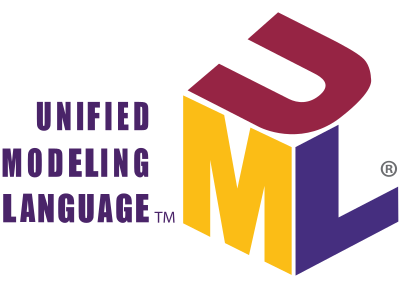
\includegraphics[width=0.3\textwidth]{pictures/web/UML_logo.svg.png}
\caption{UML Official Logo}
\label{fig:uml_logo}
\end{figure}

UML's key differentiators include comprehensive standardization, broad industry acceptance, and robust tooling ecosystem. While specialized languages such as BPMN address business process modeling and SysML serves systems engineering, UML delivers extensive coverage for software-intensive system development \cite{uml_comparison}.
\section{Conclusion}

This chapter established the foundation for developing an intelligent UML diagram generation platform by addressing critical challenges in current diagramming approaches. The analysis revealed significant limitations in both traditional GUI-based tools and textual specification methods, highlighting the need for innovative solutions that combine precision with accessibility.

Our proposed platform leverages artificial intelligence and natural language processing to bridge these gaps, offering intelligent requirement interpretation and automated diagram generation through PlantUML integration. The selection of Scrum methodology ensures structured yet flexible development approach suitable for complex AI-driven projects, while UML's comprehensive standardization provides the necessary foundation for diverse modeling requirements.

The combination of proven technologies (PlantUML), established methodologies (Scrum), and innovative AI integration positions this project to deliver significant value to software development communities. The platform's focus on collaboration and community building creates sustainable ecosystem for knowledge sharing and continuous improvement in diagram-driven development practices.
